\documentclass[tikz,border=0pt]{standalone}
%% Shared style for the figures: TUHH colour palette, Latin Modern fonts.
%% Highlights are bold at caption size (10 pt); longer text is regular and
%% 2 pt smaller (8 pt). Figures are drawn at the text width of the
%% manuscript (390 pt) and must be included unscaled.
\usepackage[T1]{fontenc}
\usepackage{lmodern}
\usepackage{graphicx}
\usepackage{tikz}
\usetikzlibrary{arrows.meta,positioning,calc,fit,backgrounds}

\definecolor{tuhhturquoise}{HTML}{00C1D4}
\definecolor{tuhhyellow}{HTML}{FFDE36}
\definecolor{tuhhred}{HTML}{FF4F4F}
\definecolor{tuhhmint}{HTML}{5AFFC5}
\definecolor{tuhhcoolgray}{HTML}{D0D0CE}
\definecolor{tuhhpurple}{HTML}{7200FE}
\definecolor{tuhhwarmgray}{HTML}{A8968C}
\colorlet{ink}{black!85}

\newcommand{\hl}[1]{{\fontsize{10}{12}\selectfont\bfseries #1}}
\newcommand{\tx}[1]{{\fontsize{8}{9.6}\selectfont #1}}
\newcommand{\txi}[1]{{\fontsize{8}{9.6}\selectfont\itshape #1}}

%% \logo{file stem}{height}{fallback wordmark}: uses logos/<stem>.pdf or
%% .png when present, and a typeset wordmark otherwise.
\newcommand{\logo}[3]{%
  \IfFileExists{logos/#1.pdf}{\includegraphics[height=#2]{logos/#1.pdf}}{%
  \IfFileExists{logos/#1.png}{\includegraphics[height=#2]{logos/#1.png}}{%
  {\fontsize{10}{12}\selectfont\bfseries\sffamily #3}}}}

\tikzset{
  x=1pt, y=1pt, text=ink,
  card/.style={draw=tuhhcoolgray, line width=0.8pt, rounded corners=3pt,
               fill=white},
  band/.style={rounded corners=3pt, draw=none},
  flow/.style={-{Stealth[length=5pt,width=4.5pt]}, line width=1pt,
               draw=ink},
  gap/.style={draw=tuhhred, line width=1pt, dash pattern=on 3pt off 2pt},
  lbl/.style={inner sep=0pt, outer sep=0pt, align=left, anchor=north west},
  tag/.style={fill=tuhhyellow, rounded corners=2pt, inner xsep=3pt,
              inner ysep=1.5pt, anchor=west},
}

\begin{document}
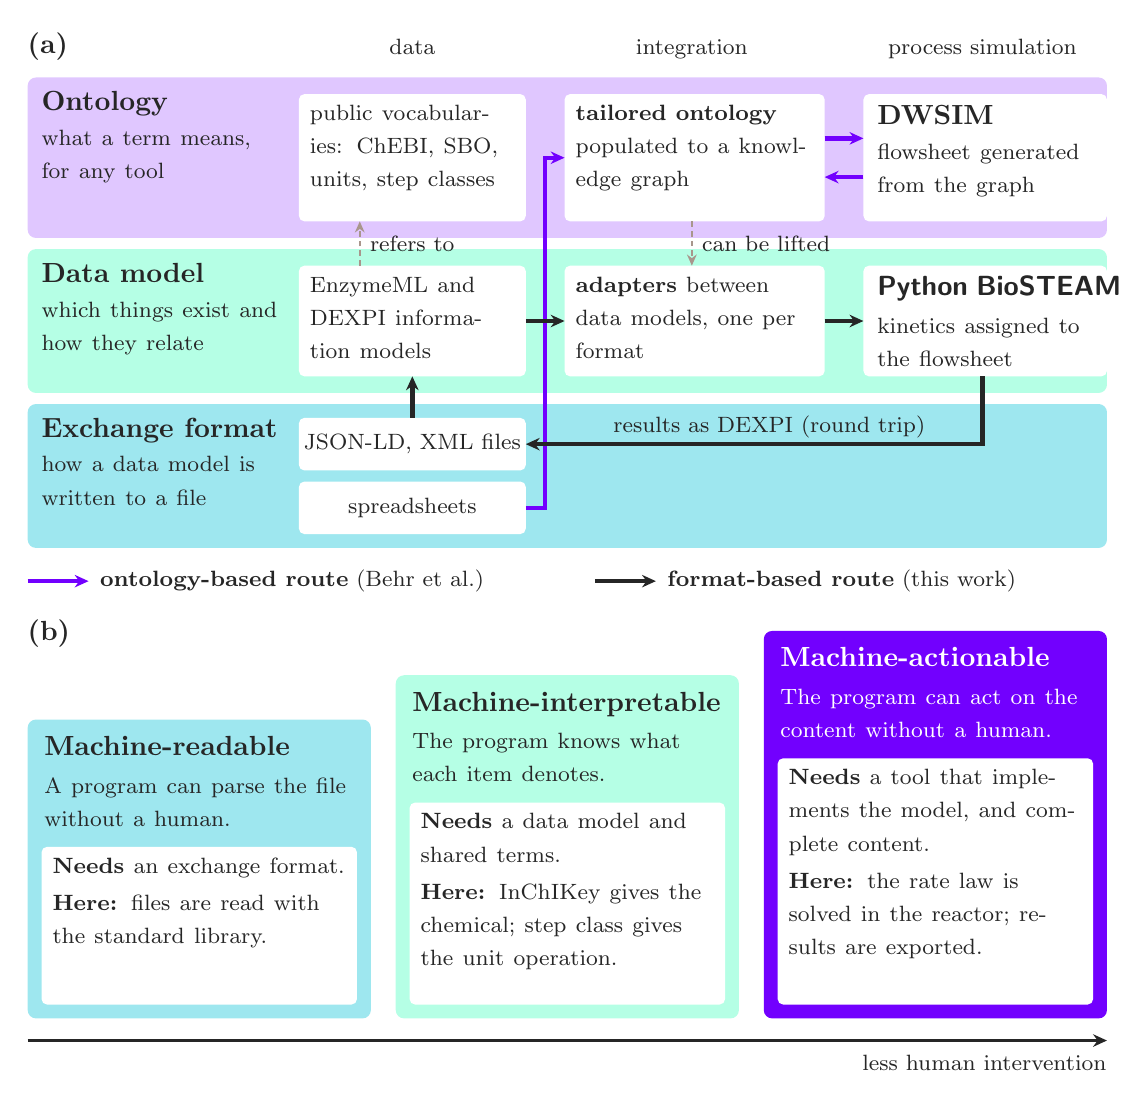
\begin{tikzpicture}
\useasboundingbox (0,0) rectangle (390,382);
\tikzset{
  cell/.style={fill=white, rounded corners=2pt, draw=none},
  routeA/.style={-{Stealth[length=5pt,width=4.5pt]}, line width=1.6pt,
                 draw=tuhhpurple},
  routeB/.style={-{Stealth[length=5pt,width=4.5pt]}, line width=1.6pt,
                 draw=ink},
  refers/.style={-{Stealth[length=4pt,width=3.5pt]}, line width=0.8pt,
                 draw=tuhhwarmgray, dash pattern=on 2pt off 1.5pt},
}

% ===========================================================================
% (a) two routes across the three levels
% ===========================================================================
\node[lbl] at (0,380) {\hl{(a)}};
\node[anchor=north, inner sep=0pt] at (139,378) {\tx{data}};
\node[anchor=north, inner sep=0pt] at (240,378) {\tx{integration}};
\node[anchor=north, inner sep=0pt] at (345,378) {\tx{process simulation}};

% level bands
\fill[band, tuhhpurple!22] (0,306) rectangle (390,364);
\fill[band, tuhhmint!45] (0,250) rectangle (390,302);
\fill[band, tuhhturquoise!38] (0,194) rectangle (390,246);
\node[lbl] at (5,359) {\hl{Ontology}};
\node[lbl, text width=86pt] at (5,345) {\tx{what a term means, for any tool}};
\node[lbl] at (5,297) {\hl{Data model}};
\node[lbl, text width=86pt] at (5,283) {\tx{which things exist and how they relate}};
\node[lbl] at (5,241) {\hl{Exchange format}};
\node[lbl, text width=86pt] at (5,227) {\tx{how a data model is written to a file}};

% cells, column 1 (x 98-180)
\fill[cell] (98,312) rectangle (180,358);
\node[lbl, text width=74pt] at (102,354)
  {\tx{public vocabularies: ChEBI, SBO, units, step classes}};
\fill[cell] (98,256) rectangle (180,296);
\node[lbl, text width=74pt] at (102,292)
  {\tx{EnzymeML and DEXPI information models}};
\fill[cell] (98,222) rectangle (180,241);
\node[anchor=center] at (139,231.5) {\tx{JSON-LD, XML files}};
\fill[cell] (98,199) rectangle (180,218);
\node[anchor=center] at (139,208.5) {\tx{spreadsheets}};

% cells, column 2 (x 194-288)
\fill[cell] (194,312) rectangle (288,358);
\node[lbl, text width=86pt] at (198,354)
  {\tx{\textbf{tailored ontology} populated to a knowledge graph}};
\fill[cell] (194,256) rectangle (288,296);
\node[lbl, text width=86pt] at (198,292)
  {\tx{\textbf{adapters} between data models, one per format}};

% simulators (x 302-390)
\fill[cell] (302,312) rectangle (390,358);
\node[lbl] at (307,354) {\hl{DWSIM}};
\node[lbl, text width=78pt] at (307,340) {\tx{flowsheet generated from the graph}};
\fill[cell] (302,256) rectangle (390,296);
\node[lbl] at (307,292) {\logo{python}{11pt}{Python}\hspace{3pt}\logo{biosteam}{10pt}{BioSTEAM}};
\node[lbl, text width=78pt] at (307,277) {\tx{kinetics assigned to the flowsheet}};

% route A: ontology-based (Behr et al.)
\draw[routeA] (180,208.5) -- (187,208.5) -- (187,335) -- (194,335);
\draw[routeA] (288,342) -- (302,342);
\draw[routeA] (302,328) -- (288,328);

% route B: format-based (this work)
\draw[routeB] (139,241) -- (139,256);
\draw[routeB] (180,276) -- (194,276);
\draw[routeB] (288,276) -- (302,276);
\draw[routeB] (345,256) -- (345,231.5) -- (180,231.5);
\node[anchor=south, inner sep=1.5pt] at (268,232) {\tx{results as DEXPI (round trip)}};

% references to shared terms
\draw[refers] (120,296) -- (120,312);
\draw[refers] (240,312) -- (240,296);
\node[anchor=west, inner sep=1.5pt] at (122,304) {\tx{refers to}};
\node[anchor=west, inner sep=1.5pt] at (242,304) {\tx{can be lifted}};

% legend
\draw[routeA] (0,182) -- (22,182);
\node[anchor=west, inner sep=0pt] at (26,182)
  {\tx{\textbf{ontology-based route} (Behr et al.)}};
\draw[routeB] (205,182) -- (227,182);
\node[anchor=west, inner sep=0pt] at (231,182)
  {\tx{\textbf{format-based route} (this work)}};

% ===========================================================================
% (b) what a machine can do with a file
% ===========================================================================
\node[lbl] at (0,168) {\hl{(b)}};
\newcommand{\step}[8]{%
  \fill[band, #3] (#1,24) rectangle (#1+124,#2);
  \node[lbl, text=#4] at (#1+6,#2-6) {\hl{#5}};
  \node[lbl, text=#4, text width=112pt] at (#1+6,#2-21) {\tx{#6}};
  \fill[cell] (#1+5,29) rectangle (#1+119,#2-46);
  \node[lbl, text width=106pt] at (#1+9,#2-50)
    {\tx{\textbf{Needs} #7.}\\[1.5pt]\tx{\textbf{Here:} #8.}};
}
\step{0}{132}{tuhhturquoise!38}{ink}{Machine-readable}
  {A program can parse the file without a human.}
  {an exchange format}
  {files are read with the standard library}
\step{133}{148}{tuhhmint!45}{ink}{Machine-interpretable}
  {The program knows what each item denotes.}
  {a data model and shared terms}
  {InChIKey gives the chemical; step class gives the unit operation}
\step{266}{164}{tuhhpurple}{white}{Machine-actionable}
  {The program can act on the content without a human.}
  {a tool that implements the model, and complete content}
  {the rate law is solved in the reactor; results are exported}
\draw[flow] (0,16) -- (390,16);
\node[anchor=north east, inner sep=0pt] at (390,11)
  {\tx{less human intervention}};
\end{tikzpicture}
\end{document}
